\documentclass[11pt]{article}
\usepackage[margin=2.5cm]{geometry}
\usepackage{graphicx,booktabs,hyperref,amsmath}
\usepackage[T1]{fontenc}
\hypersetup{colorlinks=true,linkcolor=black,urlcolor=blue,citecolor=black}
\newcommand{\am}{$'$}
\title{Is Almagest Virgo 17 Uranus seen by Hipparchus?\\A pre-registered position test}
\author{Qianghao Wu}
\date{November 28, 2026}
\begin{document}
\sloppy
\maketitle

\begin{abstract}
K.\,P.~Hertzog (1988) proposed that the 17th star of Virgo in Ptolemy's star catalogue (Baily no.~513; longitude Virgo $27\tfrac14^\circ$, latitude $+0\tfrac16^\circ$, magnitude 6), usually identified with 76~Virginis, is the planet Uranus, observed by Hipparchus near 25 March $-127$. N.\,M.~Swerdlow (2020) wrote that he does not know how to decide the question. We tested the identification by position only, with a protocol that we committed to git before we computed any distance. We moved the entry into the frame of Hipparchus with the median offset of 266 securely identified zodiacal entries. We then compared two distances with the errors of the catalogue itself: the distance from the entry to the nearest real star with $V\le6.0$, and the smallest distance from the entry to Uranus on the nights of 149--127~BC with solar elongation of at least $120^\circ$. The reference errors are those of 103 faint identified entries (median 32.1\am, 95th percentile 88.5\am). The nearest star is 76~Vir at 63.7\am, at the 88.3rd percentile. Uranus passes 36.6\am{} from the entry on 128~BC April~7, at the 56.3rd percentile. Support for Hertzog required the star above the 95th percentile and Uranus at or below the 50th. Neither the support rule nor the refutation rule is met, so the registered result is inconclusive. In a registered placebo, 6 of 108 identified entries near the ecliptic come as close to the Uranus track; 6 of the 31 entries inside the longitude range of the track do. Uranus passes equally close (37.7\am) in Ptolemy's own time, so position alone also does not separate a Hipparchan from a Ptolemaic origin. An independent recomputation with another precession model gives the same verdict.
This work has not yet been reviewed by experts. The analysis, the code and the text were produced by AI models (from Anthropic and OpenAI), working under the author's direction.
\end{abstract}

\section{Introduction}
Uranus varies between about magnitude 5.4 and 6~\cite{swerdlow2020}. In principle it can be seen with the unaided eye under a dark sky. W.~Herschel recognised it as a new body in 1781. After that, astronomers searched older star catalogues for positions that were in fact Uranus. Swerdlow~\cite{swerdlow2020} reviews this history, from Bode's search of Tycho's catalogue to the telescopic sightings before 1781.

Hertzog~\cite{hertzog1988} proposed a much older sighting. In the summary of Swerdlow~\cite[p.~144]{swerdlow2020}, the 17th star of Virgo in Ptolemy's catalogue, ``longitude Virgo $27\tfrac14^\circ$, latitude $+0\tfrac16^\circ$, magnitude 6, doubtfully identified as 76(h) Virgo, then at longitude 179;21$^\circ$, latitude $-0$;18$^\circ$ [\ldots] is actually Uranus, observed, not by Ptolemy, but by Hipparchus, possibly on or near 25 March $-127$, when Uranus was at longitude 175;12$^\circ$, latitude $+0$;45$^\circ$''. Swerdlow's note~4 adds three facts. Hertzog uses Baily's numbering (B513) and prefers the longitude Virgo $27^\circ$. The text can be in error by $1^\circ$ in longitude or by north for south in latitude. And ``any decision rests upon first determining whether the coordinates of this star were adapted from Hipparchus. I do not know how to do this.'' Swerdlow's own answer to his title question is ``probably not, or it cannot be answered''.

Two lines of earlier work bear on the question. Verbunt and van Gent~\cite{verbunt2012} identified each entry of Ptolemy's catalogue with a Hipparcos star and published the identifications as a machine-readable table~\cite{vizierVvG}. They identify B513 with 76~Vir (HIP~66098, $V=5.2$) at a distance of 71.2\am, with their flag for a secure identification ($I=1$). The origin of the catalogue coordinates is an old debate. A recent example is Baiget Orts~\cite{baiget2026}, who dates the catalogue from the correlation between proper motions and position errors and finds a result consistent with a Hipparchan origin. That paper does not treat Uranus.

We searched for an earlier test of B513 against an ephemeris on 2026 November 28: the two public collections of AI-produced research results (clank-lab and solved-conjectures), the archives where such results are posted, Zenodo, and the web. We found Swerdlow's chapter, a popular article of 2025 that repeats the claim without a test, and the general dating work above. We found no test that judges the Uranus match against the error distribution of the catalogue. We did not read Hertzog's paper: the scan at the NASA Astrophysics Data System did not load (HTTP 500 and time-outs in two attempts on 2026 November 28). We did not check the papers that cite it.

This paper does not answer Swerdlow's question of origin. It answers a narrower one: does Uranus fit the entry better than any real naked-eye star, when both are judged by the errors that the catalogue makes for real stars?

\section{Data}
\begin{itemize}
\item \textbf{Ptolemy's catalogue}: VizieR table J/A+A/544/A31/ptolema~\cite{vizierVvG} of Verbunt and van Gent~\cite{verbunt2012}. It has 1028 entries with Toomer's values of longitude, latitude and magnitude, the Hipparcos identification (HIP), and an identification flag $I$. Accessed 2026 November 28 from the VizieR mirror at \url{https://vizier.cfa.harvard.edu}.
\item \textbf{Hipparcos}: the main catalogue (ESA 1997~\cite{hipparcos}, VizieR I/239/hip\_main), all 9827 stars with $V<6.6$ and a position: position, proper motion, parallax and $V$.
\item \textbf{Uranus}: JPL Horizons~\cite{horizons}, target 7 (Uranus barycentre), ephemeris DE441~\cite{park2021}. Geocentric ecliptic longitude and latitude of date (IAU76/80 model) and the Sun--observer--target elongation, daily at 0\,h TT. Hipparchus window: JD 1667365.5 to 1675400.5 (149~BC Dec~31 to 127~BC Dec~31, Julian calendar). Ptolemy window: JD 1764887.5 to 1774384.5 (AD~120 Jan~1 to AD~146 Jan~1).
\end{itemize}
We write years BC in historical numbering. The astronomical year $-127$ is 128~BC.

\section{Method}
\subsection{Registration}
The protocol (\texttt{PROTOCOL.md} in the result folder) was committed at 2026-11-28 01:02:27 CET. The first output of the analysis was written at 01:03:00, and the outcome was committed at 01:04:42 (\texttt{data/GIT\_LOG.txt}). Before the commit we had seen Swerdlow's numbers, the Verbunt--van Gent rows for Virgo, and the first two rows of the Horizons file, which hold no position near the entry. An addendum, added after the run, corrects a comment on the epoch (below) and lists the exploratory computations. No rule changed.

\subsection{Frame of Hipparchus}
The epoch is $t_0=$ JD 1674487.5. This is 129~BC July~1; the protocol comment ``about $-127$ January~1'' was wrong, and the code used the JD as written. We moved each Hipparcos star from epoch J1991.25 to $t_0$ with its proper motion (astropy \texttt{apply\_space\_motion}~\cite{astropy2022}; parallax $\le0$ replaced by 0.1~mas; radial velocity 0) and transformed it to the geocentric mean ecliptic and equinox of $t_0$.

The calibration set $C$ contains the entries with $I=1$, a HIP number, $|\beta_P|\le10^\circ$, and not entry 513. It has 266 entries. The frame offset is the median difference ``Ptolemy minus star'': $\Delta\lambda=+2.545^\circ$, $\Delta\beta=+0.022^\circ$. Its size, 2;33$^\circ$, is close to the difference of $-2$;40$^\circ$ in longitude that Swerdlow names for a catalogue adapted from Hipparchus~\cite[n.~4]{swerdlow2020}. The position of an entry in the Hipparchus frame is $(\lambda_P-\Delta\lambda,\ \beta_P-\Delta\beta)$. For B513 it is $(174.705^\circ, +0.145^\circ)$.

\subsection{Reference distribution and test}
The reference distribution $R$ is the set of angular distances between the entries of $C$ with Ptolemy magnitude code $\ge5$ and their identified stars, in the Hipparchus frame. It has 103 entries: 81 of magnitude 5, 21 of magnitude 6, and one entry (B577, in Sagittarius) with the code 9. In this table the code 9 occurs on Ptolemy's nebulous objects, for example Praesepe (B449); we could not retrieve the ReadMe that defines it. The protocol fixed ``code $\ge5$'', so the entry stays in $R$. Section~\ref{sec:posthoc} gives the result without it.

For B513 we computed two distances.
\begin{itemize}
\item $r_\star$: the distance to the nearest Hipparcos star with $V\le6.0$, any star, not only 76~Vir.
\item $d_U$: the smallest distance to Uranus over the days of the Hipparchus window with elongation $\ge120^\circ$ (2491 days).
\end{itemize}
$Q_S$ and $Q_U$ are their percentiles in $R$: the percentage of $R$ that is at or below the value.

The decision rule was fixed before the run:
\begin{itemize}
\item \textbf{Support} for Hertzog: $Q_S>95$ and $Q_U\le50$.
\item \textbf{Refutation} (Uranus not favoured): $Q_S\le Q_U$, or $Q_U>95$.
\item Otherwise \textbf{inconclusive}.
\end{itemize}

\subsection{Controls}
\begin{itemize}
\item \textbf{Placebo.} For each entry of $C$ with $|\beta_P|\le3^\circ$ (108 entries) we computed the same $d_U$. $F$ is the fraction with $d_U$ at or below that of B513. If $F>0.2$, the Uranus match alone is weak evidence.
\item \textbf{Known answer.} 200 fake entries made from Uranus positions on random days of the window. The pipeline must recover each within 1\am.
\item \textbf{Frame check.} The residuals of $C$ must correlate with the distances of Verbunt and van Gent (Spearman $\rho>0.8$).
\item \textbf{Secondary, descriptive.} The same computation with the epoch AD~136 December~23 (JD 1771088.5) and the Ptolemy window.
\end{itemize}

\section{Result}
Table~\ref{tab:main} gives the registered numbers. Figure~\ref{fig:main} shows the sky near the entry and the reference distribution.

\begin{table}[h]
\centering\small
\begin{tabular}{lr}\toprule
Quantity (Hipparchus window) & Value \\\midrule
Calibration entries $|C|$; frame offset $\Delta\lambda$, $\Delta\beta$ & 266; $+2.545^\circ$, $+0.022^\circ$ \\
Reference set $R$: size, median, 95th percentile & 103, 32.1\am, 88.5\am \\
Nearest star with $V\le6.0$ & 76 Vir (HIP 66098, $V=5.21$) \\
$r_\star$, $Q_S$ & 63.7\am, 88.3 \\
$d_U$, $Q_U$ & 36.6\am, 56.3 \\
Night of $d_U$; elongation & 128~BC Apr~7 (JD 1674767.5); $161^\circ$ \\
Uranus on that night & $174.704^\circ$, $+0.754^\circ$ \\
Placebo: entries with $d_U\le36.6$\am & 6 of 108 ($F=0.056$) \\
Known answer: largest recovered distance (200 cases) & $5\times10^{-5}$\am \\
Spearman $\rho$ with Verbunt--van Gent distances & 0.93 \\
\midrule
Verdict & inconclusive \\\bottomrule
\end{tabular}
\caption{Registered result. Source: \texttt{data/expected.json}, key \texttt{analysis.hipparchus}.}
\label{tab:main}
\end{table}

\begin{figure}[h]
\centering
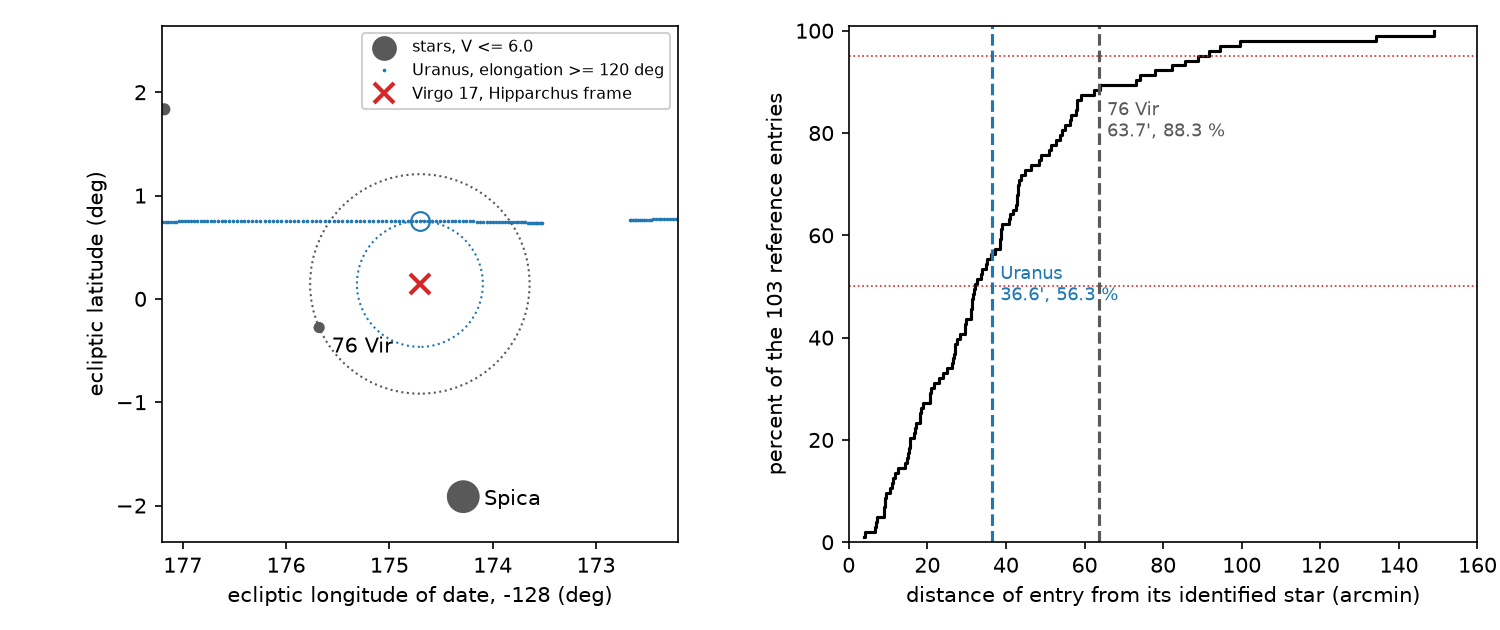
\includegraphics[width=\textwidth]{fig_virgo17.png}
\caption{Left: the sky near Virgo 17 in the frame of Hipparchus (ecliptic of JD 1674487.5). Red cross: the entry after removal of the frame offset. Blue dots: Uranus on the window days with elongation $\ge120^\circ$; open circle: the closest night, 128~BC Apr~7. Grey dots: Hipparcos stars with $V\le6.0$, size by brightness. Dotted circles: radius $d_U=36.6$\am{} (blue) and $r_\star=63.7$\am{} (grey). Right: cumulative distribution of the 103 reference distances, with the two distances of the entry. Dotted red lines: the 50th and 95th percentiles of the rule. Made by \texttt{checks/figure.py}.}
\label{fig:main}
\end{figure}

$Q_S=88.3$ is not above 95, so the support rule fails. $Q_S>Q_U$ and $Q_U\le95$, so the refutation rule also fails. The result is inconclusive.

Three facts describe the two candidates.
\begin{itemize}
\item 76~Vir is not beyond the 95th percentile of the reference errors. 12 of the 103 reference entries have a larger error. Its offset from the entry is $-58.5$\am{} in longitude and $+25.3$\am{} in latitude (entry minus star).
\item The Uranus distance is an ordinary catalogue error. It is almost all in latitude: the entry is 36.6\am{} south of Uranus. Near this longitude Uranus was at latitude $+0.73^\circ$ to $+0.76^\circ$; the entry is at $+0.14^\circ$.
\item On 128~BC March~25, the date that Hertzog names, Horizons gives Uranus at $175.24^\circ$, $+0.757^\circ$, elongation $174^\circ$. Swerdlow gives 175;12$^\circ$ ($175.20^\circ$), $+0$;45$^\circ$, $173^\circ$.
\end{itemize}

\textbf{Placebo.} The six entries that come as close to the Uranus track are B432 (Gem~9), B456 (Cnc~8), B469 (Leo~8, Regulus), B485 (Leo~24), B491 (Leo~30) and B502 (Vir~6). All are real stars with secure identifications. $F=6/108=0.056$ is below the registered limit 0.2.

\textbf{Ptolemy window (descriptive).} With Ptolemy's own epoch and AD 120--146, the offset is $\Delta\lambda=-1.110^\circ$, $\Delta\beta=+0.048^\circ$. 76~Vir is at 63.8\am{} ($Q=87.4$). Uranus passes 37.7\am{} from the entry on AD~125 March~24 ($Q=56.3$), and the placebo gives 8 of 108. Position alone does not separate the two epochs.

\section{Post hoc limits}\label{sec:posthoc}
The following numbers were computed after the result, to answer the issues of the verification round. They are not part of the decision. They come from \texttt{checks/posthoc.py} in the same frame as the registered test (\texttt{data/expected.json}, key \texttt{posthoc}).

\textbf{Placebo inside the track.} With elongation $\ge120^\circ$, Uranus covers only longitudes $79.2^\circ$ to $182.1^\circ$ in the window. 77 of the 108 placebo entries lie outside this range (with a margin of $1^\circ$) and cannot match. Of the 31 entries inside the range, 6 match: 0.19. This is still below the limit 0.2, but close to it. The Uranus match is therefore specific at the 6\,\% level only among all ecliptic entries; among entries that Uranus could reach, about one in five matches as well.

\textbf{Reference set.} Without the code-9 entry B577 (102 entries), $Q_S=88.2$ and $Q_U=55.9$. With the 21 entries of magnitude 6 only, $Q_S=81.0$ and $Q_U=47.6$.

\textbf{Sampling error of the percentiles.} In 5000 bootstrap samples of $R$ (seed 1), the 95\,\% interval of $Q_S$ is 81.6 to 94.2, and that of $Q_U$ is 46.6 to 66.0. $Q_S$ exceeds 95 in 1.2\,\% of the samples. In the frame of the independent recomputation (Section~\ref{sec:checks}) the interval of $Q_S$ is 82.5 to 95.1.

\textbf{Longitude Virgo $27^\circ$.} The test used Toomer's longitude 177;15$^\circ$. Hertzog prefers 177;00$^\circ$~\cite[n.~4]{swerdlow2020}. With 177;00$^\circ$ and latitude $+0$;10$^\circ$, 76~Vir is at 77.7\am{} ($Q=91.3$) and Uranus at 36.4\am{} ($Q=56.3$). With 177;00$^\circ$ and the variant latitude $-0$;10$^\circ$, 76~Vir is at 73.7\am{} ($Q=90.3$) and Uranus at 56.4\am{} ($Q=82.5$). With 177;15$^\circ$ and $-0$;10$^\circ$, Uranus is at 56.6\am{} and 76~Vir at 58.7\am{} (\texttt{checks/exploratory.py}). No variant meets the support rule.

\textbf{Elongation cut.} With a cut of $90^\circ$ or $150^\circ$, $d_U$ stays 36.6\am. Without a cut it is 32.4\am, on a day with solar elongation below $90^\circ$.

\textbf{Identification flag.} $R$ uses only entries that Verbunt and van Gent flag as secure ($I=1$). They give B513 itself the flag $I=1$ with 76~Vir. Swerdlow calls the identification doubtful.

\section{How the results were checked}\label{sec:checks}
\begin{itemize}
\item \textbf{Rerun.} \texttt{checks/rerun.py} downloads the three raw data sets again and recomputes every number of this paper. It compares 120 values (63 registered and exploratory values, 57 post hoc values) with \texttt{data/expected.json}, with a relative tolerance of $10^{-6}$. The rerun from a clean copy of the result folder gave a full match (\texttt{NUMBERS.md}).
\item \textbf{Independent recomputation.} The verification stage wrote new code from the protocol, without the analysis code (\texttt{checks/verify/indep.py}). It moves the stars with linear motion of unit vectors and the long-term precession matrix of Vondr\'ak et al.\ (ERFA \texttt{ltecm}), and rotates Horizons geocentric ICRF vectors of Uranus and the Sun with the same matrix. It gives $\Delta\lambda=+2.549^\circ$, $\Delta\beta=+0.021^\circ$; $R$ with 103 entries, median 32.2\am, 95th percentile 88.4\am; 76~Vir at 64.0\am{} ($Q_S=89.3$); Uranus at 36.5\am{} ($Q_U=56.3$) on the same night; placebo 6 of 108. The verdict is the same. The largest difference, 0.3\am, comes from the precession model; one reference entry lies between 63.7\am{} and 64.0\am, so $Q_S$ moves by one entry. This comparison also bounds the difference between the astropy ecliptic used for the stars and the Horizons ecliptic used for Uranus.
\item \textbf{Dates.} The verification stage converted the Julian dates with its own calendar function. JD 1674487.5 is 129~BC July~1 and JD 1674767.5 is 128~BC April~7.
\end{itemize}

\section{Limits}
\begin{itemize}
\item We did not read Hertzog's paper. His claim is quoted from Swerdlow~\cite{swerdlow2020}. We did not check the papers that cite Hertzog.
\item The test uses position only. It does not use the brightness of Uranus, the visibility of a magnitude-6 object, or the prior rarity of a planet among the catalogue entries.
\item The test does not decide whether the coordinates of B513 come from Hipparchus. The Uranus distance is the same in both windows.
\item The reference distribution has 103 entries, so each percentile has a sampling error of several points (Section~\ref{sec:posthoc}).
\item The meaning of magnitude code 9 in the VizieR table is not confirmed from its ReadMe.
\item The Uranus distance is a minimum over 2491 nights, while the star distance has no such free choice. The protocol accepts this asymmetry; the placebo measures how often a minimum of this kind is small by chance.
\item In an exploratory computation we found a ratio of 7.0 between the empirical densities of the reference distances at 36.6\am{} and at 63.7\am. The width of the window for this ratio (8\am) was chosen after the result, and the ratio ignores the free choice of date and the prior. We do not use it as evidence.
\end{itemize}

\section{Conclusion}
By position alone, Virgo 17 does not decide between Uranus and 76~Vir. Uranus fits at an ordinary catalogue error. 76~Vir fits at a large error, but not beyond the 95th percentile of the faint entries. A Uranus match of this quality occurs for about one in five catalogue entries that lie on the track. A decision needs evidence other than the position of this one entry, for example Swerdlow's question of the origin of the coordinates.

\section*{Data and code}
All code, the protocol, the expected values and the commit list are in the result folder: \url{https://github.com/KenWuqianghao/kenwu-lab/tree/main/results/almagest-virgo-uranus}. \texttt{bash checks/ci.sh} reruns everything from the public data.

\section*{Acknowledgements}
This research has made use of the VizieR catalogue access tool, CDS, Strasbourg, France, and of the JPL Horizons system. We thank F.~Verbunt and R.\,H.~van Gent for the identification table, and N.\,M.~Swerdlow for the open-access chapter that states the question.

\begin{thebibliography}{10}
\bibitem{hertzog1988} K.\,P.~Hertzog, ``Ancient Uranus?'', Quarterly Journal of the Royal Astronomical Society 29, 277--279 (1988). ADS 1988QJRAS..29..277H. Not read; cited as reported in~\cite{swerdlow2020}, note~4.
\bibitem{swerdlow2020} N.\,M.~Swerdlow, ``A curiosity: Did Ptolemy see Uranus?'', in A.~Jones and C.~Carman (eds.), \emph{Instruments -- Observations -- Theories: Studies in the History of Astronomy in Honor of James Evans}, 143--146 (2020), doi:\href{https://doi.org/10.5281/zenodo.3975731}{10.5281/zenodo.3975731}. CC BY 4.0.
\bibitem{verbunt2012} F.~Verbunt and R.\,H.~van Gent, ``The star catalogues of Ptolemaios and Ulugh Beg'', A\&A 544, A31 (2012), doi:\href{https://doi.org/10.1051/0004-6361/201219596}{10.1051/0004-6361/201219596}.
\bibitem{vizierVvG} F.~Verbunt and R.\,H.~van Gent, VizieR catalogue J/A+A/544/A31, ``Star catalogues of Ptolemaios, Ulugh Beg'', doi:\href{https://doi.org/10.26093/cds/vizier.35440031}{10.26093/cds/vizier.35440031}. Accessed 2026 Nov 28.
\bibitem{hipparcos} ESA, \emph{The Hipparcos and Tycho Catalogues}, ESA SP-1200 (1997); VizieR catalogue I/239. Accessed 2026 Nov 28.
\bibitem{horizons} JPL Horizons system, API \url{https://ssd.jpl.nasa.gov/api/horizons.api}. Accessed 2026 Nov 28.
\bibitem{park2021} R.\,S.~Park, W.\,M.~Folkner, J.\,G.~Williams, D.\,H.~Boggs, ``The JPL Planetary and Lunar Ephemerides DE440 and DE441'', AJ 161, 105 (2021), doi:\href{https://doi.org/10.3847/1538-3881/abd414}{10.3847/1538-3881/abd414}.
\bibitem{astropy2022} Astropy Collaboration, A.\,M.~Price-Whelan, P.\,L.~Lim, et al., ``The Astropy Project: Sustaining and Growing a Community-oriented Open-source Project and the Latest Major Release (v5.0) of the Core Package'', ApJ 935, 167 (2022), doi:\href{https://doi.org/10.3847/1538-4357/ac7c74}{10.3847/1538-4357/ac7c74}.
\bibitem{baiget2026} C.~Baiget Orts, ``Speed-Error Cross-Correlation Dating of Ancient Star Catalogues, with Application to the Almagest'', arXiv:\href{https://arxiv.org/abs/2604.02521}{2604.02521} (2026).
\end{thebibliography}
\end{document}
